\ifdefined\standalone 
\documentclass[12pt]{article}
\usepackage{graphicx}
\usepackage{float}
\usepackage[a4paper, margin=1in]{geometry}
\usepackage[utf8]{inputenc}
\usepackage{textcomp}
\usepackage{amsmath}
\usepackage{booktabs}
\usepackage{tikz}
\usepackage{enumitem}
\usetikzlibrary{decorations.pathmorphing,patterns}
\usepackage[hidelinks]{hyperref} % <- hypertext
\usepackage{caption}

\begin{document}
\fi

\section{In-depth radiation absorption}

This verification case is designed to assess the capability of \textt{Gpyro} to accurately model one-dimensional radiative heat absorption in a semi-opaque material. A slab of thickness $10~\mathrm{cm}$ is subjected exclusively to an incident radiative heat flux of $q''_{\mathrm{ext}} = 5~\mathrm{kW\,m^{-2}}$, which penetrates the material. The slab is assumed to be semi-opaque and characterized by a constant absorption coefficient $\kappa = 24~\mathrm{m^{-1}}$. Under these assumptions, the volumetric radiative heat source resulting from in-depth radiation absorption is described by an Beer-Lambert law:
\begin{equation}
\dot{Q}''_r(z) = \varepsilon \kappa q''_{\mathrm{ext}} \exp\left( -\kappa z \right)
\end{equation}
where $z$ denotes the distance from the irradiated surface and $\varepsilon$ is the surface emissivity.
Three configurations are considered: radiation applied at the top surface, at the bottom surface, and at both surfaces simultaneously. For each case, numerical results (annotated Gpyro latest) are compared with the corresponding analytical solution and with results obtained using the original version of \texttt{Gpyro} (annotated Gpyro V0.8). The thermophysical properties and simulation parameters are listed in Table~\ref{tab:simu_props_raddepth}.


\begin{table}[H]
\centering
\small
\caption{Simulation properties}
\label{tab:simu_props_raddepth}
\renewcommand{\arraystretch}{1.3}
\begin{tabular}{c c c c c c}
\hline
$k$ ($\mathrm{W\,m^{-1}\,K^{-1}}$) & 
$c_p$ ($\mathrm{J\,kg^{-1}\,K^{-1}}$) & 
$\rho$ ($\mathrm{kg\,m^{-3}}$) & 
$\varepsilon$ ($-$) &
$\kappa$ ($\mathrm{m^{-1}}$) &
$q''_{\mathrm{ext}}$ ($\mathrm{kW\,m^{-2}}$) \\
\hline
0.10 & 1000 & 100 & 1.0 & 24 & 5 \\
\hline
\end{tabular}
\end{table}


\begin{figure}[H]
\centering

% ---- First row ----
\begin{minipage}[t]{0.48\textwidth}
\centering
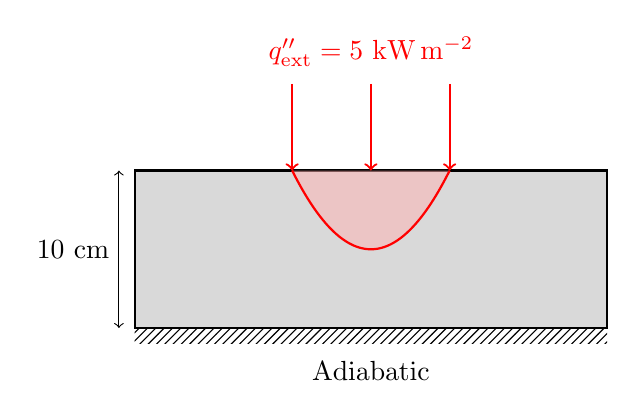
\begin{tikzpicture}[scale=1.0]
% Slab
\draw[fill=gray!30,thick] (0,0) rectangle (6,2);

% Adiabatic bottom
\fill[pattern=north east lines] (0,-0.2) rectangle (6,0);
\node[below] at (3,-0.3) {Adiabatic};

% Thickness
\draw[<->] (-0.2,0) -- (-0.2,2);
\node[left] at (-0.2,1) {10~cm};

% Incident radiation
\foreach \x in {1.8,2.8,3.8}
  \draw[->,thick,red] (\x+0.2,3.1) -- (\x+0.2,2);

\node[above,red] at (3,3.2) {$q''_{\mathrm{ext}} = 5~\mathrm{kW\,m^{-2}}$};

% Absorption profile
\fill[red!30, opacity=0.5, domain=2:4, variable=\x]
  (2,2) plot ({\x}, {(\x-3)^2 + 1}) -- (4,2) -- cycle;

\draw[thick, red, domain=2:4, samples=100]
  plot ({\x}, {(\x-3)^2 + 1});
\end{tikzpicture}
\caption*{(a) Configuration schematic}
\end{minipage}
\hfill
\begin{minipage}[t]{0.48\textwidth}
\centering
\includegraphics[width=\linewidth]{top_flux_results.png}
\caption*{(b) Top irradiation}
\end{minipage}

\begin{minipage}[t]{0.48\textwidth}
\centering
\includegraphics[width=\linewidth]{bottom_flux_results.png}
\caption*{(c) Bottom irradiation}
\end{minipage}
\hfill
\begin{minipage}[t]{0.48\textwidth}
\centering
\includegraphics[width=\linewidth]{double_flux_results.png}
\caption*{(d) Double-sided irradiation}
\end{minipage}

\caption{Comparison between Gpyro and analytical solutions for in-depth radiation.}
\label{fig:flow_comparison}
\end{figure}



\ifdefined\standalone
\end{document}
\fi






